\documentclass[uplatex,a4paper,dvipdfmx]{jsarticle} % upLaTeX と jsarticle を使用する場合

% LuaLaTeX と ltjsarticle を使用する場合
% \documentclass{ltjsarticle}

% LuaLaTeX と bxjsarticle を使用する場合
% \documentclass[lualatex]{bxjsarticle}
% \usepackage{luatexja}
% \usepackage[ipa]{luatexja-preset}

% XeLaTeX と bxjsarticle を使用する場合
% \documentclass[xelatex,ja=standard]{bxjsarticle}
% \usepackage{zxjatype}

\usepackage{lcutrinko}

\usepackage[top=10truemm,bottom=15truemm,left=10truemm,right=10truemm,headheight=0truemm,headsep=0truemm,footskip=10truemm]{geometry}
% bxjsarticle を使用する場合は以下
% \setpagelayout{top=0truemm,bottom=5truemm,left=10truemm,right=10truemm}

\usepackage{tabularx} % 表の幅を自動調整するためのもの
\usepackage{graphicx}

\begin{document}

\title{A Study of Denkikei's History\\電気系の歴史の研究}
\date{明治6年1月1日}
\author{01-234567 電気太郎}
\rinkotype{成果輪講資料}
\laboratory{指導教員: ウィリアム・エドワード・エアトン教授}

\dendentitle

\begin{abstract}
  東大電気系は明治6年(1873年)に創設された工部省工学寮電信科を起源とする学科です.
\end{abstract}

\section{最近のできごと}

以下のTable~\ref{tab:history}に今世紀の電気系の主なできごとを記す.

\begin{table}[htbp]
  \centering
  \caption{Some important events of EEIS in this century}
  \label{tab:history}
  \begin{tabularx}{\linewidth}{r|X}
    年度 & できごと \\\hline
    2001 & 大学院情報理工学系研究科(電子情報学専攻)の新設 \\
    2005 & 工学部新2号館の竣工 \\
    2008 & 電気工学専攻、電子工学専攻、基盤情報学専攻から電気系工学専攻への改組\\
    2009 & 電気工学科、電子工学科から電気電子工学科への改組\\
  \end{tabularx}
\end{table}

\section{エアトン先生}

ウィリアム・エドワード・エアトン先生(Fig.~\ref{fig:ayrton})は電気系の最初の教授です.

\begin{figure}[htbp]
  \centering
  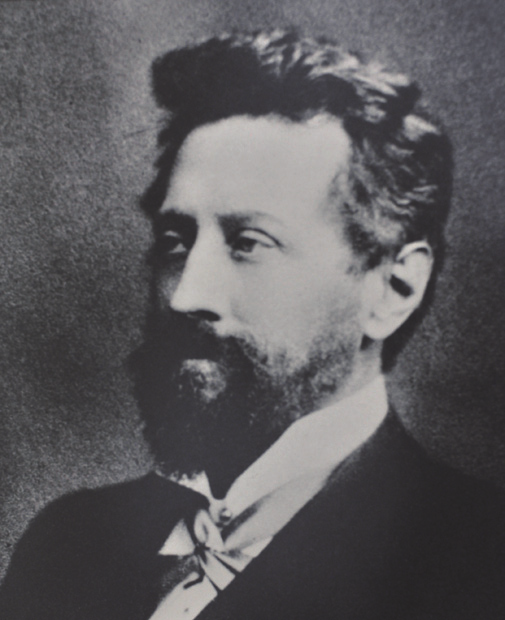
\includegraphics[height=45truemm]{ayrton.png}
  \caption{Prof. W. E. Ayrton}
  \label{fig:ayrton}
\end{figure}

\begin{thebibliography}{9}
\bibitem{guidance} 東京大学工学部電気電子工学科・電子情報工学科事務室『進学ガイダンスブック2016』
\end{thebibliography}


\end{document}